\documentclass[tikz,convert={outfile=images/liftFree-nat.png,density=1000}]{standalone}
\usepackage{xcolor}
\usepackage[build={latexoptions={-output-directory=latex/png}}]{standalone}
\begin{document}
\tikzstyle{every node}=[font=\footnotesize]
\tikzset{
  ->/.style={draw=white!50!black,-stealth}
}
\tikzstyle{every node}=[color=white!50!black,font=\tiny]
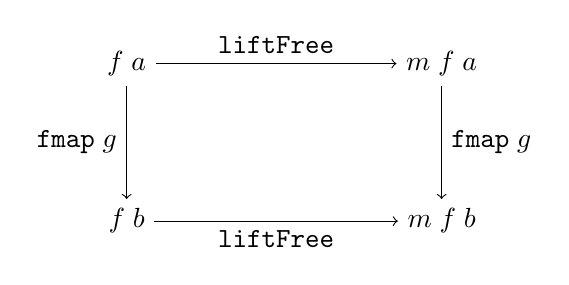
\begin{tikzpicture}
    \node (A) at (0,2) {\texttt{$f\;a$}};
    \node (B) at (4,2) {\texttt{$m\;f\;a$}};
    \node (C) at (0,0) {\texttt{$f\;b$}};
    \node (D) at (4,0) {\texttt{$m\;f\;b$}};
    \draw[->] (A) -- node[left] {$\texttt{fmap}\;g$} (C);
    \draw[->] (B) -- node[right] {$\texttt{fmap}\;g$} (D);
    \draw[->] (A) -- node [above] {$\texttt{liftFree}$} (B);
    \draw[->] (C) -- node [below] {$\texttt{liftFree}$} (D);
\end{tikzpicture}
\end{document}
